%% Submissions for peer-review must enable line-numbering 
%DIF LATEXDIFF DIFFERENCE FILE


%% using the lineno option in the \documentclass command.
%%
%% Preprints and camera-ready submissions do not need 
%% line numbers, and should have this option removed.
%%
%% Please note that the line numbering option requires
%% version 1.1 or newer of the wlpeerj.cls file, and
%% the corresponding author info requires v1.2

\documentclass[fleqn,10pt,lineno]{wlpeerj} % for journal submissions
% \documentclass[fleqn,10pt]{wlpeerj} % for preprint submissions

%DIF 14a14-15
\usepackage{float} %DIF > 
\floatplacement{figure}{H} %DIF > 
%DIF -------
\title{Spatial variation in allometric growth of invasive lionfish has
management implications}

\author[1]{Juan Carlos Villaseñor-Derbez}
\author[1]{Sean Fitzgerald}
\affil[1]{Bren School of Environmental Sciences and Management, University of California
  Santa Barbara, Santa Barbara, California, USA}
%DIF 21c23
%DIF < \corrauthor[1]{Juan Carlos Villaseñor-Derbez}{jvillasenor@ucsb.edu}
%DIF -------
\corrauthor[1]{Juan Carlos Villaseñor-Derbez}{juancarlos@ucsb.edu} %DIF > 
%DIF -------

\keywords{Lionfish, invasive species, length-weight, allometric, regional variations}

\begin{abstract}
Lionfish (\textit{Pterois volitans / miles}) are an invasive species in
the Western Atlantic and the Caribbean. Improving management of invasive
lionfish populations requires accurate total biomass estimates, which
%DIF 29c31
%DIF < depend on accurate estimates of allometric growth. Sedentary species
%DIF -------
depend on accurate estimates of allometric growth, but sedentary species %DIF > 
%DIF -------
like lionfish often exhibit high levels of spatial variation in life
%DIF 31c33
%DIF < history characteristics. We review 17 published length-weight
%DIF -------
history characteristics. We reviewed 17 published length-weight %DIF > 
%DIF -------
relationships for lionfish taken throughout their invasive range and
%DIF 33-41c35-44
%DIF < found substantial regional differences in allometric growth parameters.
%DIF < The spatial pattern we observed is consistent with findings from other
%DIF < studies focusing on genetics or age-at-length. We show that the use of
%DIF < \textit{ex situ} parameters can result in up to a threefold under- or
%DIF < overestimation of total weight, but using parameters from nearby regions
%DIF < reduces this error. These findings can have major implications for
%DIF < management in terms of predicting effects on local ecosystems,
%DIF < evaluating the effectiveness of removal programs, or estimating biomass
%DIF < available for harvest.
%DIF -------
found regional differences that led to significant misestimates when %DIF > 
calculating weight from length observations. The spatial pattern we %DIF > 
observed is consistent with findings from other studies focused on %DIF > 
genetics or length-at-age. Here, the use of \textit{ex situ} parameter %DIF > 
values resulted in total biomass estimates between 76.2\% and 140\% of %DIF > 
true observed biomass, and up to a threefold under- or overestimation of %DIF > 
total weight for an individual organism. These findings can have %DIF > 
implications for management in terms of predicting effects on local %DIF > 
ecosystems, evaluating the effectiveness of removal programs, or %DIF > 
estimating biomass available for harvest. %DIF > 
%DIF -------
\end{abstract}
%DIF PREAMBLE EXTENSION ADDED BY LATEXDIFF
%DIF UNDERLINE PREAMBLE %DIF PREAMBLE
\RequirePackage[normalem]{ulem} %DIF PREAMBLE
\RequirePackage{color}\definecolor{RED}{rgb}{1,0,0}\definecolor{BLUE}{rgb}{0,0,1} %DIF PREAMBLE
\providecommand{\DIFadd}[1]{{\protect\color{blue}\uwave{#1}}} %DIF PREAMBLE
\providecommand{\DIFdel}[1]{{\protect\color{red}\sout{#1}}}                      %DIF PREAMBLE
%DIF SAFE PREAMBLE %DIF PREAMBLE
\providecommand{\DIFaddbegin}{} %DIF PREAMBLE
\providecommand{\DIFaddend}{} %DIF PREAMBLE
\providecommand{\DIFdelbegin}{} %DIF PREAMBLE
\providecommand{\DIFdelend}{} %DIF PREAMBLE
%DIF FLOATSAFE PREAMBLE %DIF PREAMBLE
\providecommand{\DIFaddFL}[1]{\DIFadd{#1}} %DIF PREAMBLE
\providecommand{\DIFdelFL}[1]{\DIFdel{#1}} %DIF PREAMBLE
\providecommand{\DIFaddbeginFL}{} %DIF PREAMBLE
\providecommand{\DIFaddendFL}{} %DIF PREAMBLE
\providecommand{\DIFdelbeginFL}{} %DIF PREAMBLE
\providecommand{\DIFdelendFL}{} %DIF PREAMBLE
%DIF END PREAMBLE EXTENSION ADDED BY LATEXDIFF

\begin{document}

\flushbottom
\maketitle
\thispagestyle{empty}

\section*{Introduction}

Lionfish (\emph{Pterois volitans/miles} complex) are an invasive species
in the \DIFdelbegin \DIFdel{western Atlantic }\DIFdelend \DIFaddbegin \DIFadd{Western Atlantic Ocean }\DIFaddend and Caribbean Sea, likely introduced
through \DIFdelbegin \DIFdel{liberation }\DIFdelend \DIFaddbegin \DIFadd{release }\DIFaddend of aquarium-kept organisms \citep{betancurr_2011}.
\DIFdelbegin \DIFdel{They }\DIFdelend \DIFaddbegin \DIFadd{Lionfish }\DIFaddend are the first invasive marine vertebrates established along
\DIFdelbegin \DIFdel{the North
Atlantic Caribbean coasts \mbox{%DIFAUXCMD
\citep{schofield_2009,schofield_2010,sabidoitza_2016}}\hspace{0pt}%DIFAUXCMD
and their }\DIFdelend \DIFaddbegin \DIFadd{these coasts \mbox{%DIFAUXCMD
\citep{schofield_2009,schofield_2010,sabidoitza_2016}}\hspace{0pt}%DIFAUXCMD
, and
they have established invasive populations in coral reefs, estuaries,
mangroves, hard-bottomed areas, and mesophotic reefs
\mbox{%DIFAUXCMD
\citep{barbour_2010,jud_2011,muoz_2011,claydon_2012,andradibrown_2017,gress_2017}}\hspace{0pt}%DIFAUXCMD
.
Their }\DIFaddend presence has been labeled as a \DIFaddbegin \DIFadd{``}\DIFaddend major marine invasion\DIFaddbegin \DIFadd{'' }\DIFaddend because
they threaten local biodiversity, spread rapidly, and are difficult to
manage \citep{hixon_2016}.
\DIFdelbegin \DIFdel{Lionfish have established invasive populations in
coral reefs, estuaries, mangroves, hard-bottomed areas, and mesophotic
reefs
\mbox{%DIFAUXCMD
\citep{barbour_2010,jud_2011,muoz_2011,claydon_2012,andradibrown_2017,gress_2017}}\hspace{0pt}%DIFAUXCMD
.
}\DIFdelend 

A substantial amount of research describes lionfish impacts throughout
\DIFdelbegin \DIFdel{its }\DIFdelend \DIFaddbegin \DIFadd{their }\DIFaddend invaded range. A meta-analysis by \citet{peake_2018} showed that
invasive lionfish prey on at least 167 different species across the
tropical and temperate \DIFdelbegin \DIFdel{North }\DIFdelend \DIFaddbegin \DIFadd{Western }\DIFaddend Atlantic. Their feeding behavior and high
consumption rates can reduce recruitment and population sizes of native
reef-fish species, and can further endanger reef fish
\DIFdelbegin \DIFdel{(\mbox{%DIFAUXCMD
\citet{green_2012,rocha_2015}}\hspace{0pt}%DIFAUXCMD
; but see \mbox{%DIFAUXCMD
\citet{hackerott_2017}}\hspace{0pt}%DIFAUXCMD
)}\DIFdelend \DIFaddbegin \DIFadd{\mbox{%DIFAUXCMD
\citep[][but see \citealt{hackerott_2017} for a counterexample]{green_2012,rocha_2015}}\hspace{0pt}%DIFAUXCMD
}\DIFaddend .
For example, field experiments \DIFdelbegin \DIFdel{by \mbox{%DIFAUXCMD
\citet{albins_2008} }\hspace{0pt}%DIFAUXCMD
}\DIFdelend showed that lionfish establishment \DIFaddbegin \DIFadd{in the
Bahamas }\DIFaddend led to reduced recruitment of native fishes by nearly 80\% over
a five-week period \DIFdelbegin \DIFdel{in Florida. \mbox{%DIFAUXCMD
\citet{green_2012} }\hspace{0pt}%DIFAUXCMD
reported that
}\DIFdelend \DIFaddbegin \DIFadd{\mbox{%DIFAUXCMD
\citep{albins_2008}}\hspace{0pt}%DIFAUXCMD
, and }\DIFaddend prey fish biomass declined
by 65\% over two years as lionfish biomass increased along Bahamian
coral reefs \DIFdelbegin \DIFdel{. Their trophic impacts }\DIFdelend \DIFaddbegin \DIFadd{\mbox{%DIFAUXCMD
\citep{green_2012}}\hspace{0pt}%DIFAUXCMD
. However, trophic impacts of lionfish }\DIFaddend can
be minimized if \DIFdelbegin \DIFdel{local lionfish }\DIFdelend \DIFaddbegin \DIFadd{their local }\DIFaddend biomass is controlled by culling
\citep{ariasgonzalez_2011}.

Governments and non-profit organizations have sought to reduce lionfish
densities through removal programs and \DIFaddbegin \DIFadd{by }\DIFaddend incentivizing its consumption
\citep{chin_2016}. In some cases, these have shown to significantly
reduce \DIFdelbegin \DIFdel{--but not quite eliminate-- }\DIFdelend \DIFaddbegin \DIFadd{-- but not quite eliminate -- }\DIFaddend lionfish abundances at local scales
\citep{deleon_2013,sandel_2015}. Complete eradication of lionfish
through fishing is unlikely because of their rapid recovery rates and
ongoing recruitment to shallow-water areas from persistent populations
in mesophotic ecosystems \citep{barbour_2011,andradibrown_2017}.
However, promoting lionfish consumption might create a level of demand
capable of incentivizing a stable fishery while controlling
shallow-water populations, thus creating alternative livelihoods and
avoiding further \DIFdelbegin \DIFdel{impacts }\DIFdelend \DIFaddbegin \DIFadd{negative effects }\DIFaddend to local biota.

The feasibility of establishing fisheries through lionfish removal
programs has been extensively evaluated through field observations and
empirical modeling
\citep{barbour_2011,morris_2011,deleon_2013,johnston_2015,sandel_2015,usseglio_2017}.
Determining the feasibility of such initiatives requires modeling the
change in biomass in response to changes in fishing mortality
(\emph{i.e.\DIFaddbegin \DIFadd{,}\DIFaddend } culling). A common way to model this is via
length-structured population models, where fish lengths are converted to
weight to calculate total biomass
\citep{barbour_2011,cote_2014,andradibrown_2017}. The allometric
length-weight relationship is thus an essential component of these
models, but this relationship can vary across regions as a response to
biotic and abiotic conditions \citep{johnson_2016}.

Outcomes of previous studies suggest lionfish are likely to exhibit
spatial heterogeneity in the length-weight relationship \DIFdelbegin \DIFdel{, which we
summarize in two main causes. First, culling programs are effective in
reducing local adult populations largely because lionfish exhibit }\DIFdelend \DIFaddbegin \DIFadd{for both
behavioral and biological reasons. Important life history
characteristics such as growth or natural mortality rates are often
spatially variable for fish that exhibit sedentary behavior
\mbox{%DIFAUXCMD
\citep{gunderson_2008,hutchinson_2008,wilson_2012,guan_2013}}\hspace{0pt}%DIFAUXCMD
, and in
fact, }\DIFaddend high levels of site fidelity and small home ranges \DIFdelbegin \DIFdel{\mbox{%DIFAUXCMD
\citep{Fishelson_1997,kochzius_2005,jud_2012,cote_2014}}\hspace{0pt}%DIFAUXCMD
. It is know that
fish with sedentary behavior are likely to exhibit high levels of
spatial variation in important life history characterstics such as
growth or natural mortality rates
\mbox{%DIFAUXCMD
\citep{gunderson_2008,hutchinson_2008,wilson_2012,guan_2013}}\hspace{0pt}%DIFAUXCMD
. Second,
genetic }\DIFdelend \DIFaddbegin \DIFadd{are two primary
reasons why culling programs are effective in reducing local adult
lionfish populations
\mbox{%DIFAUXCMD
\citep{Fishelson_1997,kochzius_2005,jud_2012,cote_2014}}\hspace{0pt}%DIFAUXCMD
. Genetic
}\DIFaddend analysis of lionfish \DIFdelbegin \DIFdel{suggests biological differences due to the
existence of }\DIFdelend \DIFaddbegin \DIFadd{also identified }\DIFaddend two genetically distinct invasive
subpopulations between the \DIFdelbegin \DIFdel{northwest }\DIFdelend \DIFaddbegin \DIFadd{Western }\DIFaddend Atlantic and the Caribbean\DIFaddbegin \DIFadd{,
suggesting the existence of spatially explicit biological differences
between populations as well }\DIFaddend \citep{betancurr_2011}. Site-specific
\DIFdelbegin \DIFdel{parameters are necessary to accurately estimate biomass
when allometric relationships are spatially variable , and this
variability is }\DIFdelend \DIFaddbegin \DIFadd{studies that calculate the length-weight relationship of lionfish report
variable estimates, and these differences may be }\DIFaddend increasingly important
when estimating the potential effectiveness of lionfish culling programs
\citep{barbour_2011,morris_2011,cote_2014,johnston_2015}. However, the
\DIFdelbegin \DIFdel{region-wide differences in allometric growth parameters has remained
unexplored for lionfish, despite the
large number of site-specific
studies reporting the }\DIFdelend \DIFaddbegin \DIFadd{influence of using }\emph{\DIFadd{ex situ}} \DIFadd{parameters when estimating the
}\DIFaddend length-weight relationship \DIFaddbegin \DIFadd{remains unexplored}\DIFaddend .

\DIFdelbegin \DIFdel{Here, we compare previously published }\DIFdelend \DIFaddbegin \DIFadd{Our objective was to quantify the magnitude of error caused by using
}\emph{\DIFadd{ex situ}} \DIFadd{parameter values when estimating lionfish weight from
length observations. In this study, we calculated and reported the first
}\DIFaddend length-weight \DIFdelbegin \DIFdel{relationships for lionfish populations in North Carolina, Northern and Southern Gulf of
Mexico, the Southern Mexican Caribbean
, Bahamas, Little Cayman, Jamaica,
Bonaire, Puerto Rico, and Costa Rica
\mbox{%DIFAUXCMD
\citep{barbour_2011,darling_2011,deleon_2013,fogg_2013,dahl_2014,edwards_2014,toledohernndez_2014,sandel_2015,aguilarperera_2016,sabidoitza_2016,sabidoitz_2016,chin_2016}}\hspace{0pt}%DIFAUXCMD
. We also collected lionfish length and weight data in the central Mexican
Caribbean and report the first allometric growth equation for this
region. The objective of this paper is to describe the spatial pattern
of }\DIFdelend \DIFaddbegin \DIFadd{relationship for lionfish in the central Mexican Caribbean
using previously collected }\emph{\DIFadd{in situ}} \DIFadd{observations (n = 109;
\mbox{%DIFAUXCMD
\citet{villaseorderbez_2014}}\hspace{0pt}%DIFAUXCMD
). We then estimated lionfish weight in this
area using previously published }\DIFaddend length-weight relationships \DIFdelbegin \DIFdel{of lionfish
across the Caribbean and
Western Atlanticand to discuss implications of these spatial
differences}\DIFdelend \DIFaddbegin \DIFadd{for lionfish
populations from ten locations across the Western Atlantic, Gulf of
Mexico, and Caribbean. By comparing these weight estimates to our
}\emph{\DIFadd{in situ}} \DIFadd{length-weight observations, we showed that using }\emph{\DIFadd{ex
situ}} \DIFadd{parameter values resulted in up to a threefold under- or
overestimation of lionfish weight and estimated of total biomass ranged
between 76\% and 140\% of observed total biomass}\DIFaddend .

\DIFdelbegin %DIFDELCMD < \clearpage
%DIFDELCMD < 

%DIFDELCMD < %%%
\DIFdelend \section*{Methods}

We reviewed 12 published studies and obtained 17 length-weight
relationships for the \DIFdelbegin \DIFdel{North }\DIFdelend \DIFaddbegin \DIFadd{Western }\DIFaddend Atlantic (n = \DIFdelbegin \DIFdel{1}\DIFdelend \DIFaddbegin \DIFadd{2}\DIFaddend ), Gulf of Mexico (n = 7),
and Caribbean (n = \DIFdelbegin \DIFdel{9}\DIFdelend \DIFaddbegin \DIFadd{8}\DIFaddend , Table \ref{tab:all_params}, Fig \DIFdelbegin \DIFdel{\ref{fig:all_allo}).
We }\DIFdelend \DIFaddbegin \DIFadd{\ref{fig:map}).
Study sites included North Carolina, the Northern and Southern Gulf of
Mexico, the Southern Mexican Caribbean, the Bahamas, Little Cayman,
Jamaica, Bonaire, Puerto Rico, and Costa Rica
\mbox{%DIFAUXCMD
\citep{barbour_2011,darling_2011,deleon_2013,fogg_2013,dahl_2014,edwards_2014,toledohernndez_2014,sandel_2015,aguilarperera_2016,sabidoitza_2016,sabidoitz_2016,chin_2016}}\hspace{0pt}%DIFAUXCMD
.
We have access only to the summarized information published in these
studies - not the raw data authors used to make length-weight
calculations. We }\DIFaddend collected information on \DIFdelbegin \DIFdel{sampling methods, }\DIFdelend sex differentiation, location,
\DIFaddbegin \DIFadd{length }\DIFaddend and depth ranges\DIFaddbegin \DIFadd{, and sampling methods }\DIFaddend from each study when
available. Only two studies reported \DIFdelbegin \DIFdel{parameters for each gender
}\DIFdelend \DIFaddbegin \DIFadd{sex-specific length-weight
parameters }\DIFaddend \citep{aguilarperera_2016,fogg_2013}, so we assumed \DIFdelbegin \DIFdel{both genders were
included in a study if gender was unspecified}\DIFdelend \DIFaddbegin \DIFadd{data were
reported for both sexes combined in all other studies}\DIFaddend . Reviewed studies
presented information for organisms \DIFaddbegin \DIFadd{ranging from 25-475 mm in Total
Length (\(TL\)) and were }\DIFaddend obtained at depths between 0.5 m and 57 m. \DIFdelbegin \DIFdel{Three }\DIFdelend \DIFaddbegin \DIFadd{Four
}\DIFaddend studies explicitly stated that their organisms were sampled with pole
spears \citep{dahl_2014,aguilarperera_2016,chin_2016,sabidoitz_2016},
and \DIFdelbegin \DIFdel{five
}\DIFdelend \DIFaddbegin \DIFadd{six }\DIFaddend studies mentioned that some of their organisms were obtained
with pole spears (or other type of harpoon) but also hand-held nets or
fish traps
\DIFdelbegin \DIFdel{\mbox{%DIFAUXCMD
\citep{barbour_2011,fogg_2013,edwards_2014,toledohernndez_2014,sandel_2015,sabidoitza_2016,sabidoitz_2016}}\hspace{0pt}%DIFAUXCMD
,
and two }\DIFdelend \DIFaddbegin \DIFadd{\mbox{%DIFAUXCMD
\citep{barbour_2011,fogg_2013,edwards_2014,toledohernndez_2014,sandel_2015,sabidoitza_2016}}\hspace{0pt}%DIFAUXCMD
.
Two }\DIFaddend studies did not specify how organisms were sampled
\citep{darling_2011,deleon_2013}.
\DIFdelbegin \DIFdel{\mbox{%DIFAUXCMD
\citet{fogg_2013} }\hspace{0pt}%DIFAUXCMD
use spineless weight
in their calculations, so their parameters likely underestimated total
wieght. Since no spineless to total weight conversions were available,
these parameters were taken as reported.
}\DIFdelend 

\DIFdelbegin %DIFDELCMD < \begin{figure}
%DIFDELCMD < \centering
%DIFDELCMD < 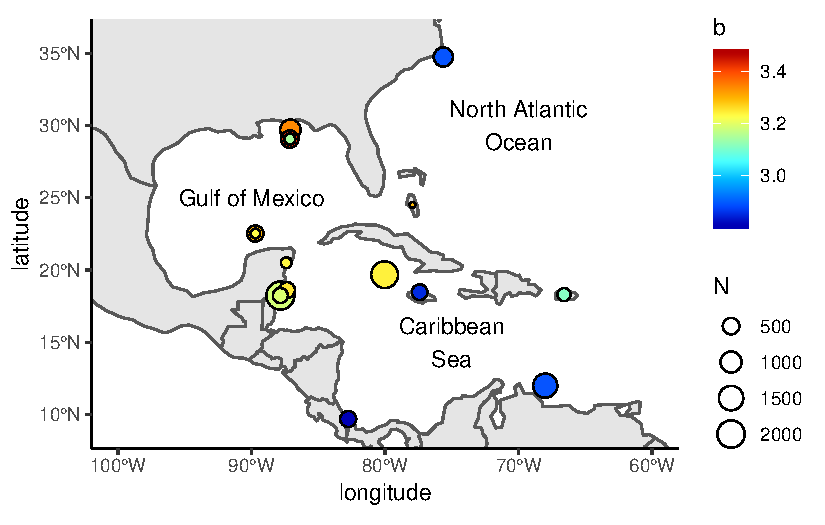
\includegraphics{Manuscript_files/figure-latex/unnamed-chunk-2-1.pdf}
%DIFDELCMD < %%%
%DIFDELCMD < \caption{%
{%DIFAUXCMD
%DIFDELCMD < \label{fig:map}%%%
\DIFdelFL{Locations where allometric growth parameters of
lionfish (}\emph{\DIFdelFL{Pterois spp}}%DIFAUXCMD
\DIFdelFL{) have been reported. Circle sizes indicate
sample size from each study, colors indicate the \(b\) coefficient from
Eq. \ref{eq:allometric}.}}
%DIFAUXCMD
%DIFDELCMD < \end{figure}
%DIFDELCMD < 

%DIFDELCMD < %%%
\DIFdel{We also collected data from }\DIFdelend \DIFaddbegin \DIFadd{We also used data from 109 lionfish sampled by
\mbox{%DIFAUXCMD
\citet{villaseorderbez_2014}}\hspace{0pt}%DIFAUXCMD
, who used hand nets and numbered bottles to
collect Total Length (TL; mm) and Total Weight (TW; g) for organisms
from }\DIFaddend 10 sampling sites along the central Mexican Caribbean coast in \DIFaddbegin \DIFadd{the
Summer of }\DIFaddend 2010 (Supplementary Table 1). Sampling locations included wall
and carpet reefs at depths between 5.7 m and 38.1 m. \DIFdelbegin \DIFdel{All
observed lionfish (n = 109) were collected using hand nets and numbered
collection bottles. }\DIFdelend The use of hand
nets prevented any weight loss due to bleeding and allowed better
representation of small sizes by \DIFdelbegin \DIFdel{eliminating }\DIFdelend \DIFaddbegin \DIFadd{avoiding }\DIFaddend gear selectivity. Organisms
were euthanized via pithing\DIFdelbegin \DIFdel{and
Total Length (TL; mm) and Total Weight (TW; g) were recorded}\DIFdelend .

\DIFaddbegin \begin{figure}
\centering
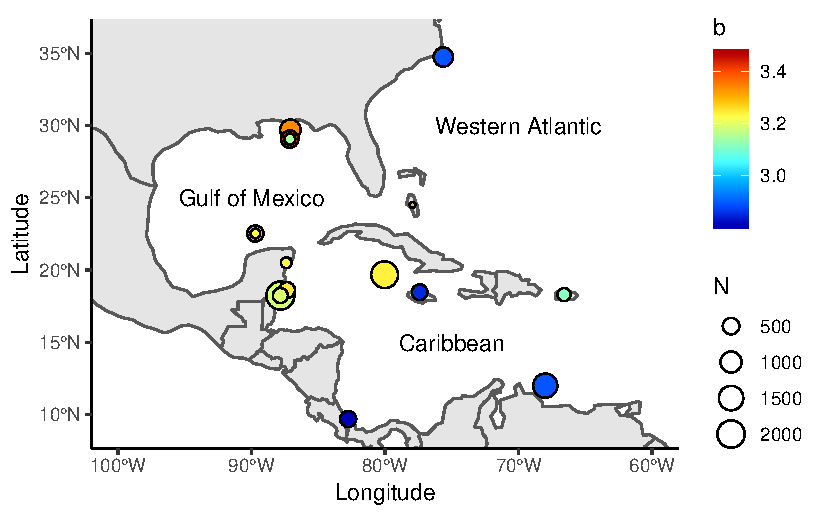
\includegraphics{Manuscript_files/figure-latex/map-1.pdf}
\caption{\label{fig:map}\DIFaddFL{Locations where allometric growth parameters of
lionfish (}\emph{\DIFaddFL{Pterois spp}}\DIFaddFL{) have been reported. Circle sizes indicate
sample size from each study, colors indicate the \(b\) coefficient from
Eq. \ref{eq:allometric}.}}
\end{figure}

\DIFaddend The weight-at-length relationship for lionfish in the central Mexican
Caribbean was calculated with the allometric growth function:

\begin{equation}
\label{eq:allometric}
TW = aTL^b
\end{equation}

Where \(a\) is the ponderal index and \(b\) is the scaling exponent or
allometric parameter. \DIFdelbegin %DIFDELCMD < 

%DIFDELCMD < \clearpage
%DIFDELCMD < 

%DIFDELCMD < %%%
\DIFdel{Transforming this equation via base-10 logarithms we obtain:
}%DIFDELCMD < 

%DIFDELCMD < %%%
\begin{displaymath}
\DIFdel{%DIFDELCMD < \label{eq:log-alo}%%%
log_{10}(TW) = b\times log_{10}(TL) + log_{10}(a)
}\end{displaymath}%DIFAUXCMD
%DIFDELCMD < 

%DIFDELCMD < %%%
\DIFdel{This can be simplified and re-written as:
}%DIFDELCMD < 

%DIFDELCMD < %%%
\begin{displaymath}
\DIFdel{%DIFDELCMD < \label{eq:log-alo-trans}%%%
Y = bX + c
}\end{displaymath}%DIFAUXCMD
%DIFDELCMD < 

%DIFDELCMD < %%%
\DIFdel{Where \(Y = log_{10}(TW)\), \(X = log_{10}(TL)\), and
\(c = log_{10}(a)\). The coefficients (\(c\) and \(b\)) were estimated with }\DIFdelend \DIFaddbegin \DIFadd{We linearized the equation using
\(log_{10}\)-transformation and estimated the coefficients using }\DIFaddend an
Ordinary Least Squares Regression \DIFdelbegin \DIFdel{and }\DIFdelend \DIFaddbegin \DIFadd{with a }\DIFaddend heteroskedastic-robust standard
error correction \citep{zeileis_2004}. \DIFdelbegin \DIFdel{When the \(b = 3\), it
is said that the organism exhibits a perfect isometric growth, so the
\(b\) coefficient was tested against the null hypothesis of isometric
growth (}\emph{\DIFdel{i.e.}} %DIFAUXCMD
\DIFdel{\(H_0: b = 3\)). }\DIFdelend Coefficients were tested with a
two-tailed Student's \DIFdelbegin \DIFdel{t}\DIFdelend \DIFaddbegin \DIFadd{t-test}\DIFaddend , and the significance of the regression was
corroborated with an F-test. \DIFdelbegin %DIFDELCMD < 

%DIFDELCMD < %%%
\DIFdelend Some of the reviewed studies \DIFaddbegin \DIFadd{(Table
\ref{tab:all_params}, Fig \ref{fig:map}) }\DIFaddend inconsistently defined \(a\) as
either the ponderal index from Eq. \ref{eq:allometric} or the
y-intercept \DIFdelbegin \DIFdel{(\(c\))
from Eq. \ref{eq:log-alo-trans}. }\DIFdelend \DIFaddbegin \DIFadd{from the linearized log-transformed equation. }\DIFaddend Other studies
incorrectly reported parameters as mm-to-g conversions when they were in
fact cm-to-g conversions. We standardized each study by converting
coefficients and report all parameters as TL (mm) to TW (\DIFdelbegin \DIFdel{gr}\DIFdelend \DIFaddbegin \DIFadd{g}\DIFaddend ) conversions.
\DIFdelbegin \DIFdel{Locations where
allometric studies have been performed are shown in Figure \ref{fig:map}
and summarized in Table \ref{tab:all_params}.
}\DIFdelend 

We obtained a total of 18 parameter pairs by combining length-weight
parameters extracted from the literature and the additional pair
calculated here \DIFdelbegin \DIFdel{. We used the central Mexican Caribbean as a case study
of
how the use of }\DIFdelend \DIFaddbegin \DIFadd{(Fig \ref{fig:all_allo}). Recall that the objective of
this study is not to describe differences in the length-weight
relationship between populations (which would require access to raw
data), but rather to assess how }\DIFaddend \emph{ex situ} \DIFdelbegin \DIFdel{parameters influences }\DIFdelend \DIFaddbegin \DIFadd{parameter values
influence }\DIFaddend the accuracy of weight estimates for lionfish\DIFdelbegin \DIFdel{. We estimated TW from the TL observations
we }\DIFdelend \DIFaddbegin \DIFadd{, using the
central Mexican Caribbean as a case study. Using each of the 18
parameter pairs, we estimated \(TW\) from the \(TL\) observations
}\DIFaddend collected in the central Mexican Caribbean (n = 109, with \DIFdelbegin \DIFdel{\(TL \in (34, 310)\)) using each of the 18 parameter pairs }\DIFdelend \DIFaddbegin \DIFadd{\(TL\) ranging
from 34 mm to 310 mm) }\DIFaddend and divided predicted weights by known observed
weights to obtain a simple measure of over- or underestimation.
Difference in mean weight ratios \DIFdelbegin \DIFdel{across the
different parameter pairs }\DIFdelend were tested with \DIFdelbegin \DIFdel{a one-way analysis of
variance (ANOVA)and }\DIFdelend \DIFaddbegin \DIFadd{an analysis of
covariance (ANCOVA):
}

\begin{equation}
\DIFadd{R_{i,j} = \tilde{\mu} + \alpha_j + \beta TL_{ij} + e_{ij}
}\end{equation}

\clearpage

\DIFadd{Where \(R_{ij}\) is the weight ratio for the \(i\)-th organism obtained
with parameters from the \(j\)-th study, \(\tilde{\mu}\) is a constant
for all individuals, \(a_j\) is the treatment effect (}\emph{\DIFadd{i.e.,}} \DIFadd{the
difference induced by each study), \(TL_{ij}\) is the covariate
(}\emph{\DIFadd{i.e.,}} \DIFadd{Total Length) for the \(i\)-th subject in the \(j\)-th
group with slope \(\beta\), and \(e_{ij}\) is the error term of the
regression. Ratios were logit-transformed prior to analysis, and a
}\emph{\DIFadd{post-hoc}} \DIFaddend Tukey's test was used \DIFdelbegin \DIFdel{for }\emph{\DIFdel{post-hoc}} %DIFAUXCMD
\DIFdel{tests}\DIFdelend \DIFaddbegin \DIFadd{to identify groups where mean
ratios did not differ}\DIFaddend . All analyses were performed in R version 3.5\DIFdelbegin \DIFdel{.1 }\DIFdelend \DIFaddbegin \DIFadd{.2
}\DIFaddend \citep{rcore_2018}. Raw data and code used in this work are available on
github \DIFdelbegin \DIFdel{.
}\DIFdelend \DIFaddbegin \DIFadd{at github.com/jcvdav/lionfish\_biometry.
}\DIFaddend 

\DIFaddbegin \begin{table}[!h]

\caption{\label{tab:unnamed-chunk-2}\label{tab:all_params}\DIFaddFL{Summary of 18 allometric growth parameters available for lionfish in the invaded range from peer-reviewed literature and this study. All parameters have been adjusted to convert from millimeters to grams. n = Sample size, Sex specifies whether data was presented for Females (F), Males (M), or both sexes combined (B), a = scaling parameter (presented in $\times 10^{-5}$), b = exponent.}}
\centering
\begin{tabular}{llllrll}
\toprule
\DIFaddFL{Region }& \DIFaddFL{Sex }& \DIFaddFL{n }& \DIFaddFL{a }& \DIFaddFL{b }& \DIFaddFL{$R^2$ }& \DIFaddFL{Reference}\\
\midrule
\DIFaddFL{Western Atlantic }& \DIFaddFL{B }& \DIFaddFL{774 }& \DIFaddFL{2.90 }& \DIFaddFL{2.89 }& \DIFaddFL{- }& \DIFaddFL{Barbour et al., 2011}\\
\DIFaddFL{Western Atlantic }& \DIFaddFL{B }& \DIFaddFL{- }& \DIFaddFL{0.25 }& \DIFaddFL{3.29 }& \DIFaddFL{- }& \DIFaddFL{Darling et al., 2011}\\
\DIFaddFL{GoM }& \DIFaddFL{B }& \DIFaddFL{934 }& \DIFaddFL{0.21 }& \DIFaddFL{3.34 }& \DIFaddFL{0.98 }& \DIFaddFL{Dahl \& Patterson, 2014}\\
\DIFaddFL{GoM }& \DIFaddFL{B }& \DIFaddFL{472 }& \DIFaddFL{0.29 }& \DIFaddFL{3.30 }& \DIFaddFL{0.95 }& \DIFaddFL{Aguilar-Perera \& Quijano-Puerto, 2016}\\
\DIFaddFL{GoM }& \DIFaddFL{F }& \DIFaddFL{67 }& \DIFaddFL{0.12 }& \DIFaddFL{3.47 }& \DIFaddFL{0.95 }& \DIFaddFL{Aguilar-Perera \& Quijano-Puerto, 2016}\\
\DIFaddFL{GoM }& \DIFaddFL{M }& \DIFaddFL{59 }& \DIFaddFL{0.42 }& \DIFaddFL{3.23 }& \DIFaddFL{0.95 }& \DIFaddFL{Aguilar-Perera \& Quijano-Puerto, 2016}\\
\DIFaddFL{GoM }& \DIFaddFL{B }& \DIFaddFL{582 }& \DIFaddFL{0.14 }& \DIFaddFL{3.43 }& \DIFaddFL{0.99 }& \DIFaddFL{Fogg et al., 2013}\\
\DIFaddFL{GoM }& \DIFaddFL{M }& \DIFaddFL{119 }& \DIFaddFL{0.27 }& \DIFaddFL{3.31 }& \DIFaddFL{0.97 }& \DIFaddFL{Fogg et al., 2013}\\
\DIFaddFL{GoM }& \DIFaddFL{F }& \DIFaddFL{115 }& \DIFaddFL{0.68 }& \DIFaddFL{3.14 }& \DIFaddFL{0.94 }& \DIFaddFL{Fogg et al., 2013}\\
\DIFaddFL{Caribbean }& \DIFaddFL{B }& \DIFaddFL{458 }& \DIFaddFL{3.60 }& \DIFaddFL{2.81 }& \DIFaddFL{- }& \DIFaddFL{Sandel et al., 2015}\\
\DIFaddFL{Caribbean }& \DIFaddFL{B }& \DIFaddFL{419 }& \DIFaddFL{2.80 }& \DIFaddFL{2.85 }& \DIFaddFL{0.87 }& \DIFaddFL{Chin et al., 2016}\\
\DIFaddFL{Caribbean }& \DIFaddFL{B }& \DIFaddFL{1450 }& \DIFaddFL{2.30 }& \DIFaddFL{2.89 }& \DIFaddFL{0.92 }& \DIFaddFL{de Leon et al., 2013}\\
\DIFaddFL{Caribbean }& \DIFaddFL{B }& \DIFaddFL{1887 }& \DIFaddFL{0.30 }& \DIFaddFL{3.24 }& \DIFaddFL{0.97 }& \DIFaddFL{Edwards et al., 2014}\\
\DIFaddFL{Caribbean }& \DIFaddFL{B }& \DIFaddFL{2143 }& \DIFaddFL{0.52 }& \DIFaddFL{3.18 }& \DIFaddFL{0.99 }& \DIFaddFL{Sabido-Itza et al., 2016}\\
\DIFaddFL{Caribbean }& \DIFaddFL{B }& \DIFaddFL{227 }& \DIFaddFL{0.80 }& \DIFaddFL{3.11 }& \DIFaddFL{0.96 }& \DIFaddFL{Toledo-Hernández et al., 2014}\\
\DIFaddFL{Caribbean }& \DIFaddFL{B }& \DIFaddFL{449 }& \DIFaddFL{0.23 }& \DIFaddFL{3.25 }& \DIFaddFL{0.97 }& \DIFaddFL{Sabido-Itza et al., 2016b}\\
\DIFaddFL{Caribbean }& \DIFaddFL{B }& \DIFaddFL{368 }& \DIFaddFL{0.32 }& \DIFaddFL{3.19 }& \DIFaddFL{0.98 }& \DIFaddFL{Sabido-Itza et al., 2016b}\\
\DIFaddFL{Caribbean }& \DIFaddFL{B }& \DIFaddFL{109 }& \DIFaddFL{0.32 }& \DIFaddFL{3.23 }& \DIFaddFL{0.98 }& \DIFaddFL{This study}\\
\bottomrule
\end{tabular}
\end{table}

\clearpage

\DIFaddend \section*{Results}

The length-weight relationship for organisms from the central Mexican
Caribbean \DIFdelbegin \DIFdel{resulted in the coefficient values \(a = 3.2056297\times 10^{-6}\), \(b = 3.2347391\) and \(c = -5.4940866\) }\DIFdelend \DIFaddbegin \DIFadd{(Fig \ref{fig:l-w-carib}) resulted in coefficient values of
\(a = 3.205 \times 10^{-6}\) and \(b = 3.235\) }\DIFaddend (\(R^2 = 0.977\),
\DIFdelbegin \DIFdel{F(df = 1; 107)= 6928.67,
\(p < 0.001\))}\DIFdelend \DIFaddbegin \DIFadd{\(F_{1, 107} = 6928.67; p < 0.001\))}\DIFaddend . The allometric factor (\(b\)) was
significantly different from \(b = 3\) (\DIFdelbegin \DIFdel{\(t(107) = 6.04; p<0.001\))indicating }\DIFdelend \DIFaddbegin \DIFadd{\(t_{107} = 6.04; p<0.001\)),
corroborating }\DIFaddend that lionfish present allometric growth. The length-weight
coefficients estimated \DIFdelbegin \DIFdel{in this study }\DIFdelend \DIFaddbegin \DIFadd{here }\DIFaddend were within the range identified by studies
\DIFdelbegin \DIFdel{in
}\DIFdelend \DIFaddbegin \DIFadd{from }\DIFaddend other regions (Table \ref{tab:all_params}).
\DIFdelbegin \DIFdel{Figure \ref{fig:l-w-carib}
shows the relationship between TL and TW for this region, and model fit
statistics are presented in Table \ref{tab:reg_table}.
}\DIFdelend 

\begin{figure}
\centering
\DIFdelbeginFL %DIFDELCMD < 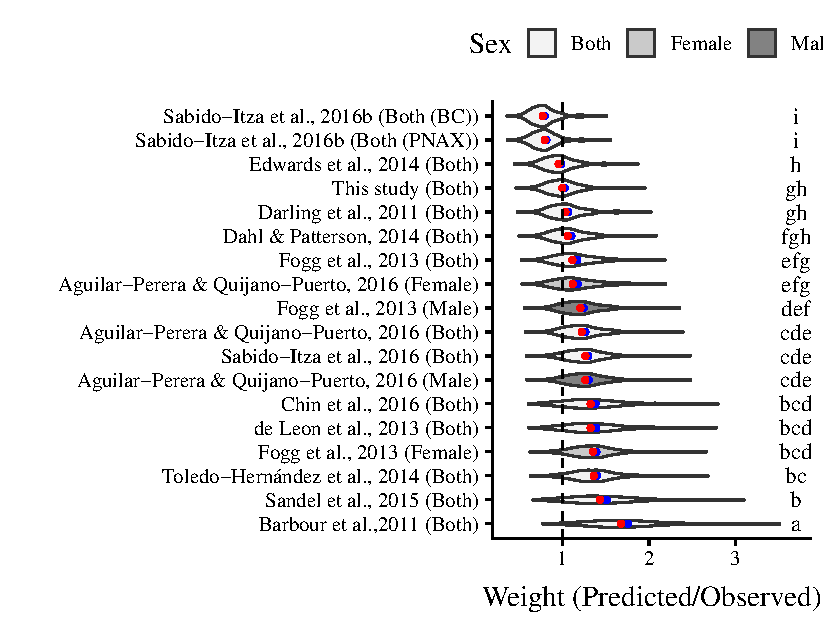
\includegraphics{Manuscript_files/figure-latex/unnamed-chunk-7-1.pdf}
%DIFDELCMD < %%%
\DIFdelendFL \DIFaddbeginFL 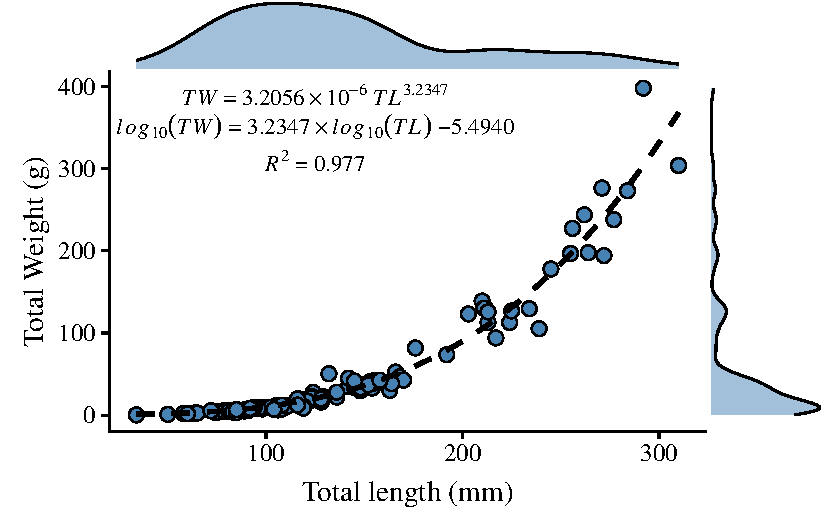
\includegraphics{Manuscript_files/figure-latex/fit1-1.pdf}
\DIFaddendFL \caption{\label{fig:l-w-carib}Length-weight relationship for 109
lionfish sampled in the central Mexican Caribbean. Points indicate
samples, dashed black line indicates curve of best fit, marginal plots
represent the density distribution of each variable.}
\end{figure}

\DIFdelbegin %DIFDELCMD < \begin{table}[!htbp] \centering 
%DIFDELCMD <   %%%
%DIFDELCMD < \caption{%
{%DIFAUXCMD
%DIFDELCMD < \label{tab:reg_table}%%%
\DIFdelFL{Coefficients of the linear model fit to Eq \ref{eq:log-alo-trans}. Numbers in parenthesees represent heteroskedastic-robust standard errors.}} 
  %DIFAUXCMD
%DIFDELCMD < \label{} 
%DIFDELCMD < \begin{tabular}{@{\extracolsep{5pt}}lc} 
%DIFDELCMD < \\[-1.8ex]\hline 
%DIFDELCMD < \hline \\[-1.8ex] 
%DIFDELCMD <  & \multicolumn{1}{c}{$log_{10}(TW)$} \\ 
%DIFDELCMD < \cline{2-2} 
%DIFDELCMD < \hline \\[-1.8ex] 
%DIFDELCMD <  %%%
\DIFdelFL{c }%DIFDELCMD < & %%%
\DIFdelFL{$-$5.494 (0.083)$^{***}$ }%DIFDELCMD < \\ 
%DIFDELCMD <   %%%
\DIFdelFL{b }%DIFDELCMD < & %%%
\DIFdelFL{3.235 (0.039)$^{***}$ }%DIFDELCMD < \\ 
%DIFDELCMD <  \hline \\[-1.8ex] 
%DIFDELCMD < %%%
\DIFdelFL{F Statistic }%DIFDELCMD < & %%%
\DIFdelFL{6928.67*** (df = 1; 107) }%DIFDELCMD < \\ 
%DIFDELCMD < %%%
\DIFdelFL{Observations }%DIFDELCMD < & %%%
\DIFdelFL{109 }%DIFDELCMD < \\ 
%DIFDELCMD < %%%
\DIFdelFL{Adjusted R$^{2}$ }%DIFDELCMD < & %%%
\DIFdelFL{0.976 }%DIFDELCMD < \\ 
%DIFDELCMD < %%%
\DIFdelFL{Residual Std. Error }%DIFDELCMD < & %%%
\DIFdelFL{0.096 (df = 107) }%DIFDELCMD < \\ 
%DIFDELCMD < \hline 
%DIFDELCMD < \hline \\[-1.8ex] 
%DIFDELCMD < %%%
\textit{\DIFdelFL{Note:}}  %DIFAUXCMD
%DIFDELCMD < & \multicolumn{1}{r}{$^{*}$p$<$0.1; $^{**}$p$<$0.05; $^{***}$p$<$0.01} \\ 
%DIFDELCMD < \end{tabular} 
%DIFDELCMD < \end{table}
%DIFDELCMD < 

%DIFDELCMD < %%%
\DIFdel{There were }\DIFdelend \DIFaddbegin \DIFadd{ANCOVA results revealed }\DIFaddend significant differences in our predicted \DIFdelbegin \DIFdel{weights }\DIFdelend \DIFaddbegin \DIFadd{weight
ratios }\DIFaddend for the central Mexican Caribbean when using \DIFaddbegin \DIFadd{each of }\DIFaddend the
different pairs of parameters (\DIFdelbegin \DIFdel{\(F(df = 17; 1944) = 61.55; p < 0.001\)). The lowest weight estimates
resulted from using the allometric parameters }\DIFdelend \DIFaddbegin \DIFadd{\(F_{17, 1943} = 24.96; p < 0.001\); Fig
\ref{fig:bio_ratio}). For example, the actual observed weights of the
109 lionfish from the Central Mexican Caribbean had a mean \(\pm\) SD of
52.56 \(\pm\) 76.58 g. However, if we used allometric parameter values
}\DIFaddend from Banco Chinchorro in the Caribbean \DIFdelbegin \DIFdel{, with }\DIFdelend \DIFaddbegin \DIFadd{to predict weights from our
observed length observations, we estimated a }\DIFaddend mean \(\pm\) SD of 40.37
\(\pm\) 58.74 \DIFdelbegin \DIFdel{gr
\mbox{%DIFAUXCMD
\citep{sabidoitz_2016}}\hspace{0pt}%DIFAUXCMD
, and the highest weight estimates came from the
Northern Atlantic with }\DIFdelend \DIFaddbegin \DIFadd{g \mbox{%DIFAUXCMD
\citep{sabidoitz_2016}}\hspace{0pt}%DIFAUXCMD
. If we similarly used parameter
values from North Carolina in the Western Atlantic to estimate lionfish
weights in the Central Mexican Caribbean, we found a mean \(\pm\) SD of
}\DIFaddend 73.76 \(\pm\) 96.11 \DIFdelbegin \DIFdel{gr \mbox{%DIFAUXCMD
\citep{barbour_2011}}\hspace{0pt}%DIFAUXCMD
. To
put this in context, true observed weights were 52.56 \(\pm\) 76.58 gr.
These correspond to }\DIFdelend \DIFaddbegin \DIFadd{g \mbox{%DIFAUXCMD
\citep{barbour_2011}}\hspace{0pt}%DIFAUXCMD
. Weights predicted from these
extreme parameters correspond to mean }\DIFaddend predicted-to-observed \DIFdelbegin \DIFdel{weights }\DIFdelend \DIFaddbegin \DIFadd{weight
}\DIFaddend ratios of 0.80 \(\pm\) 0.19 and 1.76 \(\pm\) 0.50 (mean \(\pm\) SD),
respectively. \DIFdelbegin %DIFDELCMD < 

%DIFDELCMD < %%%
\DIFdel{The calculated ratio of predicted-to-observed weight ranged from }\DIFdelend \DIFaddbegin \DIFadd{Furthermore, largest errors for individual organisms
collected in the central Mexican Caribbean resulted in ratios of }\DIFaddend 0.36
\DIFdelbegin \DIFdel{to
}\DIFdelend \DIFaddbegin \DIFadd{and }\DIFaddend 3.51 \DIFaddbegin \DIFadd{(}\emph{\DIFadd{i.e.,}} \DIFadd{the tails of each violin in Fig
\ref{fig:bio_ratio}). If we examined biomass (}\emph{\DIFadd{i.e.,}} \DIFadd{summing
across all 109 organisms) instead of mean ratios, total biomass
estimates were 76.2\% (4}\DIFaddend ,\DIFdelbegin \DIFdel{indicating that }\DIFdelend \DIFaddbegin \DIFadd{363.53 g) and 140\% (8,039.96 g) of true
observed biomass (5,729.34 g). Parameters for this study estimate total
biomass at 98\% of observed biomass. These misestimates come from the
two most extreme sets of parameters, but results varied consistently
across locations (Figs \ref{fig:bio_ratio} and \ref{fig:errors}).
Overall, the use of }\DIFaddend \emph{ex situ} parameters \DIFdelbegin \DIFdel{can result in major
under- and overestimations.
}\DIFdelend \DIFaddbegin \DIFadd{led to significantly
erroneous estimates of individual weight and total biomass for lionfish.
}

\DIFaddend Tukey's \emph{post-hoc} test \DIFdelbegin \DIFdel{suggests }\DIFdelend \DIFaddbegin \DIFadd{showed }\DIFaddend that weight ratios for the central
Mexican Caribbean \DIFdelbegin \DIFdel{were not different }\DIFdelend \DIFaddbegin \DIFadd{differeed }\DIFaddend from those obtained with parameters from \DIFdelbegin \DIFdel{Little Cayman, the Bahamas , and some
sites in the }\DIFdelend \DIFaddbegin \DIFadd{the
Western Atlantic, and most sites in the Caribbean and the Gulf of Mexico
(Tukey's HSD \(p > 0.05\)). The only sites where weight ratios did not
differ from the central Mexican Caribbean were Little Cayman
\mbox{%DIFAUXCMD
\citep{edwards_2014}}\hspace{0pt}%DIFAUXCMD
, Bahamas \mbox{%DIFAUXCMD
\citep{darling_2011}}\hspace{0pt}%DIFAUXCMD
,
and the Northern }\DIFaddend Gulf of Mexico (\DIFdelbegin \DIFdel{Tukeys }\DIFdelend \DIFaddbegin \DIFadd{\mbox{%DIFAUXCMD
\citet{dahl_2014}}\hspace{0pt}%DIFAUXCMD
; Tukey's }\DIFaddend HSD
\(p > 0.05\)). \DIFdelbegin \DIFdel{Weight }\DIFdelend \DIFaddbegin \DIFadd{All weight }\DIFaddend estimates using parameters from the Gulf of
Mexico and \DIFdelbegin \DIFdel{North-Western }\DIFdelend \DIFaddbegin \DIFadd{Western }\DIFaddend Atlantic were higher \DIFdelbegin \DIFdel{on average than those }\DIFdelend \DIFaddbegin \DIFadd{than observed values, and only
parameters }\DIFaddend from the Caribbean \DIFdelbegin \DIFdel{(Fig
\ref{fig:all_allo}}\DIFdelend \DIFaddbegin \DIFadd{produced weights smaller than observed
(Fig \ref{fig:bio_ratio}}\DIFaddend ). The \DIFaddbegin \DIFadd{regional }\DIFaddend average (\(\pm\) SD) \DIFaddbegin \DIFadd{of
}\DIFaddend predicted-to-observed weight ratios from these three regions were 1.24
\(\pm\) 0.309, \DIFdelbegin \DIFdel{1.76
}\DIFdelend \DIFaddbegin \DIFadd{1.41 }\DIFaddend \(\pm\) \DIFdelbegin \DIFdel{0.496, and 1.17 }\DIFdelend \DIFaddbegin \DIFadd{0.523, and 1.20 }\DIFaddend \(\pm\) \DIFdelbegin \DIFdel{0.398, respectively}\DIFdelend \DIFaddbegin \DIFadd{0.423 for the Gulf
of Mexico, Western Atlantic, and Caribbean, respectively. This suggests
that the smallest errors are observed when using parameters from other
locations in the Caribbean}\DIFaddend .
\DIFdelbegin \DIFdel{Predicted-to-observed weight ratios are presented in Figure
\ref{fig:bio_ratio}. Spineless weight parameters from \mbox{%DIFAUXCMD
\citet{fogg_2013}
}\hspace{0pt}%DIFAUXCMD
still produced predicted-to-observed weight ratios \textgreater{} 1.
}\DIFdelend 

\DIFdelbegin %DIFDELCMD < \begin{table}
%DIFDELCMD < 

%DIFDELCMD < %%%
%DIFDELCMD < \caption{%
{%DIFAUXCMD
%DIFDELCMD < \label{tab:unnamed-chunk-9}\label{tab:all_params}%%%
\DIFdelFL{Summary of 18 allometric growth parameters available for lionfish in the invaded range from peer-reviewed literature and this study. All parameters have been adjusted to convert from millimeters to grams. n = Sample size, Sex specifies whether data was presented for Females (F), Males (M), or both genders combined (B), a = scaling parameter for Eq. 1 (presented in $\times 10^{-5}$), c = y-intercept for Eq. 3, b = exponent or slope for Eq. 1 or Eq. 3, respectively. The Fit column contains the reported $R^2$ of the model fit.}}
%DIFAUXCMD
%DIFDELCMD < \centering
%DIFDELCMD < \begin{tabular}[t]{llllrrll}
%DIFDELCMD < \toprule
%DIFDELCMD < %%%
\DIFdelFL{Region }%DIFDELCMD < & %%%
\DIFdelFL{Sex }%DIFDELCMD < & %%%
\DIFdelFL{n }%DIFDELCMD < & %%%
\DIFdelFL{a }%DIFDELCMD < & %%%
\DIFdelFL{b }%DIFDELCMD < & %%%
\DIFdelFL{c }%DIFDELCMD < & %%%
\DIFdelFL{Fit }%DIFDELCMD < & %%%
\DIFdelFL{Reference}%DIFDELCMD < \\
%DIFDELCMD < \midrule
%DIFDELCMD < %%%
\DIFdelFL{Caribbean}%DIFDELCMD < & %%%
\DIFdelFL{B }%DIFDELCMD < & %%%
\DIFdelFL{458 }%DIFDELCMD < & %%%
\DIFdelFL{3.6 }%DIFDELCMD < & %%%
\DIFdelFL{2.81 }%DIFDELCMD < & %%%
\DIFdelFL{-4.44 }%DIFDELCMD < & %%%
\DIFdelFL{- }%DIFDELCMD < & %%%
\DIFdelFL{Sandel et al.
, 2015}%DIFDELCMD < \\
%DIFDELCMD < %%%
\DIFdelFL{Caribbean }%DIFDELCMD < & %%%
\DIFdelFL{B }%DIFDELCMD < & %%%
\DIFdelFL{419 }%DIFDELCMD < & %%%
\DIFdelFL{2.8 }%DIFDELCMD < & %%%
\DIFdelFL{2.85 }%DIFDELCMD < & %%%
\DIFdelFL{-4.56 }%DIFDELCMD < & %%%
\DIFdelFL{0.8715 }%DIFDELCMD < & %%%
\DIFdelFL{Chin et al., 2016}%DIFDELCMD < \\
%DIFDELCMD < %%%
\DIFdelFL{Caribbean }%DIFDELCMD < & %%%
\DIFdelFL{B }%DIFDELCMD < & %%%
\DIFdelFL{1450 }%DIFDELCMD < & %%%
\DIFdelFL{2.3 }%DIFDELCMD < & %%%
\DIFdelFL{2.89 }%DIFDELCMD < & %%%
\DIFdelFL{-4.64 }%DIFDELCMD < & %%%
\DIFdelFL{0.96 }%DIFDELCMD < & %%%
\DIFdelFL{de Leon et al., 2013}%DIFDELCMD < \\
%DIFDELCMD < %%%
\DIFdelFL{Caribbean }%DIFDELCMD < & %%%
\DIFdelFL{B }%DIFDELCMD < & %%%
\DIFdelFL{1887 }%DIFDELCMD < & %%%
\DIFdelFL{0.3 }%DIFDELCMD < & %%%
\DIFdelFL{3.24 }%DIFDELCMD < & %%%
\DIFdelFL{-5.52 }%DIFDELCMD < & %%%
\DIFdelFL{0.97 }%DIFDELCMD < & %%%
\DIFdelFL{Edwards et al., 2014}%DIFDELCMD < \\
%DIFDELCMD < %%%
\DIFdelFL{Caribbean }%DIFDELCMD < & %%%
\DIFdelFL{B }%DIFDELCMD < & %%%
\DIFdelFL{- }%DIFDELCMD < & %%%
\DIFdelFL{0.25 }%DIFDELCMD < & %%%
\DIFdelFL{3.29 }%DIFDELCMD < & %%%
\DIFdelFL{-5.60 }%DIFDELCMD < & %%%
\DIFdelFL{- }%DIFDELCMD < & %%%
\DIFdelFL{Darling et al., 2011}%DIFDELCMD < \\
%DIFDELCMD < \addlinespace
%DIFDELCMD < %%%
\DIFdelFL{Caribbean }%DIFDELCMD < & %%%
\DIFdelFL{B }%DIFDELCMD < & %%%
\DIFdelFL{2143 }%DIFDELCMD < & %%%
\DIFdelFL{0.52 }%DIFDELCMD < & %%%
\DIFdelFL{3.18 }%DIFDELCMD < & %%%
\DIFdelFL{-5.28 }%DIFDELCMD < & %%%
\DIFdelFL{0.9907 }%DIFDELCMD < & %%%
\DIFdelFL{Sabido-Itza et al., 2016}%DIFDELCMD < \\
%DIFDELCMD < %%%
\DIFdelFL{Caribbean }%DIFDELCMD < & %%%
\DIFdelFL{B }%DIFDELCMD < & %%%
\DIFdelFL{227 }%DIFDELCMD < & %%%
\DIFdelFL{0.8 }%DIFDELCMD < & %%%
\DIFdelFL{3.11 }%DIFDELCMD < & %%%
\DIFdelFL{-5.10 }%DIFDELCMD < & %%%
\DIFdelFL{0.958 }%DIFDELCMD < & %%%
\DIFdelFL{Toledo-Hernández et al., 2014}%DIFDELCMD < \\
%DIFDELCMD < %%%
\DIFdelFL{Caribbean }%DIFDELCMD < & %%%
\DIFdelFL{B }%DIFDELCMD < & %%%
\DIFdelFL{449 }%DIFDELCMD < & %%%
\DIFdelFL{0.23 }%DIFDELCMD < & %%%
\DIFdelFL{3.25 }%DIFDELCMD < & %%%
\DIFdelFL{-5.64 }%DIFDELCMD < & %%%
\DIFdelFL{0.97 }%DIFDELCMD < & %%%
\DIFdelFL{Sabido-Itza et al., 2016b}%DIFDELCMD < \\
%DIFDELCMD < %%%
\DIFdelFL{Caribbean }%DIFDELCMD < & %%%
\DIFdelFL{B }%DIFDELCMD < & %%%
\DIFdelFL{368 }%DIFDELCMD < & %%%
\DIFdelFL{0.32 }%DIFDELCMD < & %%%
\DIFdelFL{3.19 }%DIFDELCMD < & %%%
\DIFdelFL{-5.50 }%DIFDELCMD < & %%%
\DIFdelFL{0.98 }%DIFDELCMD < & %%%
\DIFdelFL{Sabido-Itza et al., 2016b}%DIFDELCMD < \\
%DIFDELCMD < %%%
\DIFdelFL{Caribbean }%DIFDELCMD < & %%%
\DIFdelFL{B }%DIFDELCMD < & %%%
\DIFdelFL{109 }%DIFDELCMD < & %%%
\DIFdelFL{0.32 }%DIFDELCMD < & %%%
\DIFdelFL{3.23 }%DIFDELCMD < & %%%
\DIFdelFL{-5.49 }%DIFDELCMD < & %%%
\DIFdelFL{0.9766 }%DIFDELCMD < & %%%
\DIFdelFL{This study}%DIFDELCMD < \\
%DIFDELCMD < \addlinespace
%DIFDELCMD < %%%
\DIFdelFL{GoM }%DIFDELCMD < & %%%
\DIFdelFL{B }%DIFDELCMD < & %%%
\DIFdelFL{934 }%DIFDELCMD < & %%%
\DIFdelFL{0.21 }%DIFDELCMD < & %%%
\DIFdelFL{3.34 }%DIFDELCMD < & %%%
\DIFdelFL{-5.68 }%DIFDELCMD < & %%%
\DIFdelFL{0.98 }%DIFDELCMD < & %%%
\DIFdelFL{Dahl \& Patterson, 2014}%DIFDELCMD < \\
%DIFDELCMD < %%%
\DIFdelFL{GoM }%DIFDELCMD < & %%%
\DIFdelFL{B }%DIFDELCMD < & %%%
\DIFdelFL{472 }%DIFDELCMD < & %%%
\DIFdelFL{0.29 }%DIFDELCMD < & %%%
\DIFdelFL{3.30 }%DIFDELCMD < & %%%
\DIFdelFL{-5.54 }%DIFDELCMD < & %%%
\DIFdelFL{0.95 }%DIFDELCMD < & %%%
\DIFdelFL{Aguilar-Perera \& Quijano-Puerto, 2016}%DIFDELCMD < \\
%DIFDELCMD < %%%
\DIFdelFL{GoM }%DIFDELCMD < & %%%
\DIFdelFL{F }%DIFDELCMD < & %%%
\DIFdelFL{67 }%DIFDELCMD < & %%%
\DIFdelFL{0.12 }%DIFDELCMD < & %%%
\DIFdelFL{3.47 }%DIFDELCMD < & %%%
\DIFdelFL{-5.93 }%DIFDELCMD < & %%%
\DIFdelFL{0.95 }%DIFDELCMD < & %%%
\DIFdelFL{Aguilar-Perera \& Quijano-Puerto, 2016}%DIFDELCMD < \\
%DIFDELCMD < %%%
\DIFdelFL{GoM }%DIFDELCMD < & %%%
\DIFdelFL{M }%DIFDELCMD < & %%%
\DIFdelFL{59 }%DIFDELCMD < & %%%
\DIFdelFL{0.42 }%DIFDELCMD < & %%%
\DIFdelFL{3.23 }%DIFDELCMD < & %%%
\DIFdelFL{-5.38 }%DIFDELCMD < & %%%
\DIFdelFL{0.95 }%DIFDELCMD < & %%%
\DIFdelFL{Aguilar-Perera \& Quijano-Puerto, 2016}%DIFDELCMD < \\
%DIFDELCMD < %%%
\DIFdelFL{GoM }%DIFDELCMD < & %%%
\DIFdelFL{B }%DIFDELCMD < & %%%
\DIFdelFL{582 }%DIFDELCMD < & %%%
\DIFdelFL{0.14 }%DIFDELCMD < & %%%
\DIFdelFL{3.43 }%DIFDELCMD < & %%%
\DIFdelFL{-5.86 }%DIFDELCMD < & %%%
\DIFdelFL{0.99 }%DIFDELCMD < & %%%
\DIFdelFL{Fogg et al., 2013}%DIFDELCMD < \\
%DIFDELCMD < \addlinespace
%DIFDELCMD < %%%
\DIFdelFL{GoM }%DIFDELCMD < & %%%
\DIFdelFL{M }%DIFDELCMD < & %%%
\DIFdelFL{119 }%DIFDELCMD < & %%%
\DIFdelFL{0.27 }%DIFDELCMD < & %%%
\DIFdelFL{3.31 }%DIFDELCMD < & %%%
\DIFdelFL{-5.57 }%DIFDELCMD < & %%%
\DIFdelFL{0.97 }%DIFDELCMD < & %%%
\DIFdelFL{Fogg et al., 2013}%DIFDELCMD < \\
%DIFDELCMD < %%%
\DIFdelFL{GoM }%DIFDELCMD < & %%%
\DIFdelFL{F }%DIFDELCMD < & %%%
\DIFdelFL{115 }%DIFDELCMD < & %%%
\DIFdelFL{0.68 }%DIFDELCMD < & %%%
\DIFdelFL{3.14 }%DIFDELCMD < & %%%
\DIFdelFL{-5.17 }%DIFDELCMD < & %%%
\DIFdelFL{0.94 }%DIFDELCMD < & %%%
\DIFdelFL{Fogg et al., 2013}%DIFDELCMD < \\
%DIFDELCMD < %%%
\DIFdelFL{North Atlantic }%DIFDELCMD < & %%%
\DIFdelFL{B }%DIFDELCMD < & %%%
\DIFdelFL{774 }%DIFDELCMD < & %%%
\DIFdelFL{2.9 }%DIFDELCMD < & %%%
\DIFdelFL{2.89 }%DIFDELCMD < & %%%
\DIFdelFL{-4.54 }%DIFDELCMD < & %%%
\DIFdelFL{- }%DIFDELCMD < & %%%
\DIFdelFL{Barbour et al., 2011}%DIFDELCMD < \\
%DIFDELCMD < \bottomrule
%DIFDELCMD < \end{tabular}
%DIFDELCMD < \end{table}
%DIFDELCMD < 

%DIFDELCMD < %%%
\DIFdelend \begin{figure}
\centering
\DIFdelbeginFL %DIFDELCMD < 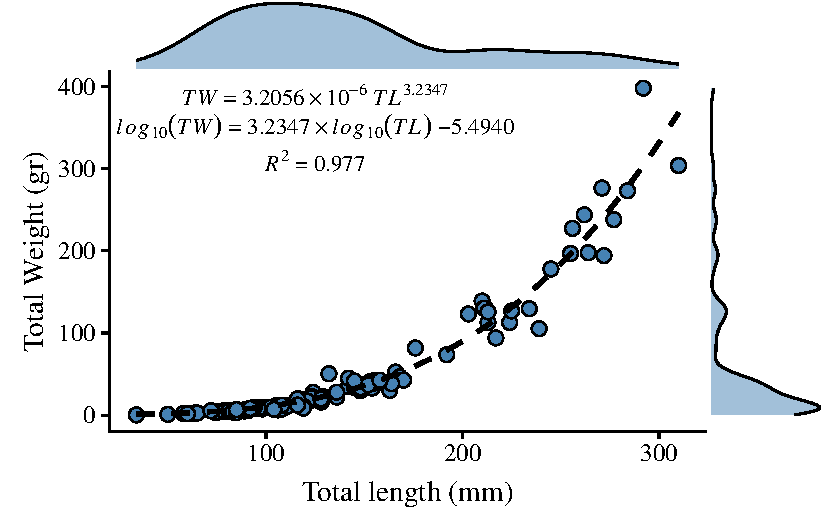
\includegraphics{Manuscript_files/figure-latex/unnamed-chunk-11-1.pdf}
%DIFDELCMD < %%%
\DIFdelendFL \DIFaddbeginFL 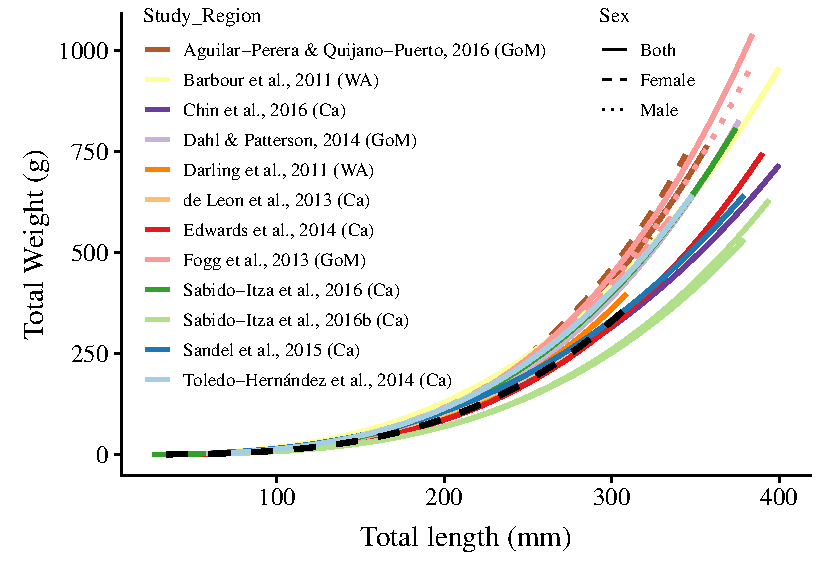
\includegraphics{Manuscript_files/figure-latex/fit2-1.pdf}
\DIFaddendFL \caption{\label{fig:all_allo}Length-weight relationships (n = 18) for 12
studies and this study. \DIFaddbeginFL \DIFaddFL{The curves are shown for the range of lengths
reported in each study (See Supplementary Table 2); when ranges were not
present, we use the ones found in this study (34 mm - 310 mm). }\DIFaddendFL Colors
indicate studies from which the parameters were extracted. Dotted,
dashed\DIFaddbeginFL \DIFaddFL{, }\DIFaddendFL and solid lines show models for males, females, and combined
sexes, respectively. \DIFaddbeginFL \DIFaddFL{Letters in parentheses indicate if the study comes
from the Gulf of Mexico (GoM), Western Atlantic (WA), or Caribbean (Ca).
}\DIFaddendFL The dashed black line represents the relationship estimated in this
study. \DIFaddbeginFL \DIFaddFL{There are two solid green lines for Sabido-Itza et al, 2016b, one
for each of the two sites for which they report parameters. A log-log
version of this figure is presented in Figure S4.}\DIFaddendFL }
\end{figure}

\begin{figure}
\centering
\DIFdelbeginFL %DIFDELCMD < 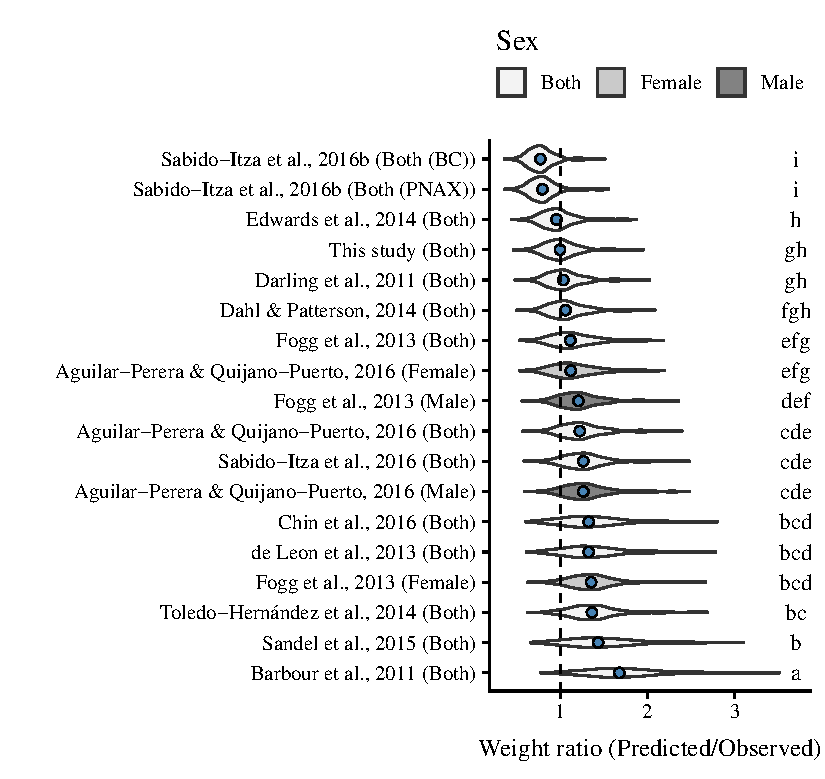
\includegraphics{Manuscript_files/figure-latex/unnamed-chunk-13-1.pdf}
%DIFDELCMD < %%%
\DIFdelendFL \DIFaddbeginFL 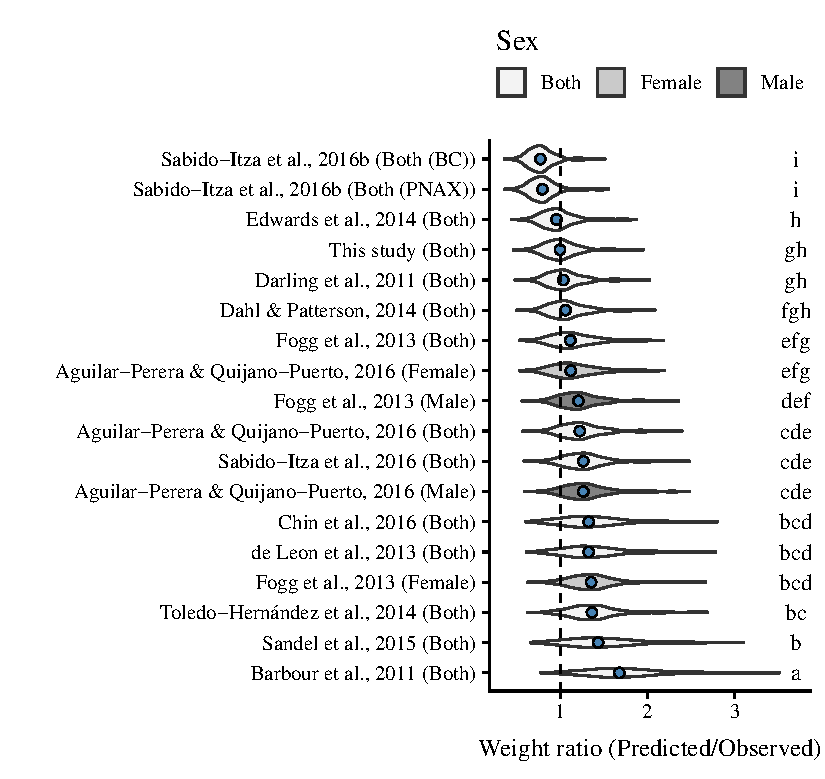
\includegraphics{Manuscript_files/figure-latex/pred_obs-1.pdf}
\DIFaddendFL \caption{\label{fig:bio_ratio}Violin plot of predicted-to-observed
weight ratios \DIFdelbeginFL \DIFdelFL{for }\DIFdelendFL \DIFaddbeginFL \DIFaddFL{when applying each of }\DIFaddendFL 18 \DIFaddbeginFL \DIFaddFL{different }\DIFaddendFL pairs of allometric
parameters \DIFaddbeginFL \DIFaddFL{to the 109 lionfish collected in the central Mexican
Caribbean}\DIFaddendFL . \DIFaddbeginFL \DIFaddFL{Sex is indicated in parentheses. }\DIFaddendFL Blue circles indicate median
values and \DIFdelbeginFL \DIFdelFL{Like }\DIFdelendFL \DIFaddbeginFL \DIFaddFL{like }\DIFaddendFL letters indicate values that do not differ
significantly. \DIFaddbeginFL \DIFaddFL{For Sabido-Itza et al, 2016b, BC and PNAX make reference
to Banco Chinchorro and Parque Nacional Arrecifes de Xcalak, two sites
for which they report parameters.}\DIFaddendFL }
\end{figure}

\DIFaddbegin \begin{figure}
\centering
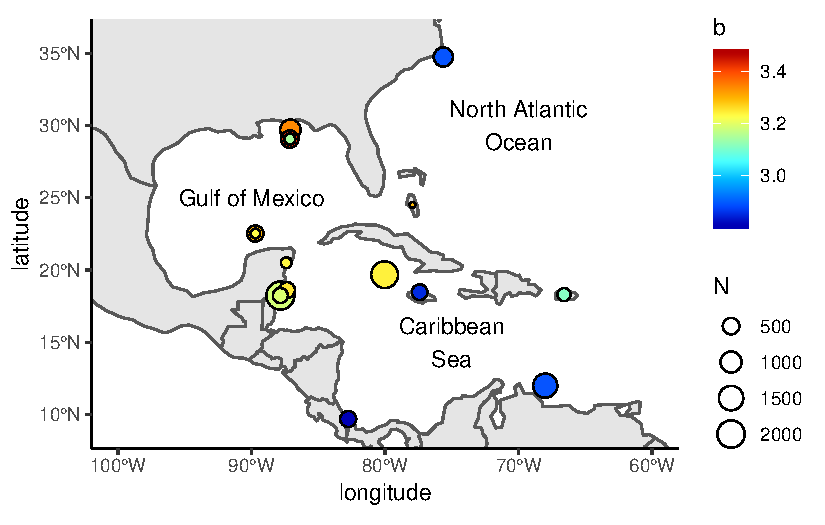
\includegraphics{Manuscript_files/figure-latex/unnamed-chunk-9-1.pdf}
\caption{\label{fig:errors}\DIFaddFL{Estimated total biomas relative to observed
biomass (5,729.34 g) for 18 pairs of allometric parameters. Sex is
indicated in parentheses. For Sabido-Itza et al, 2016b, BC and PNAX make
reference to Banco Chinchorro and Parque Nacional Arrecifes de Xcalak,
two sites for which they report parameters.}}
\end{figure}

\DIFaddend \clearpage

\section*{Discussion}

Our results suggest that lionfish exhibit highly variable\DIFaddbegin \DIFadd{, spatially
heterogeneous }\DIFaddend allometric relationships across \DIFdelbegin \DIFdel{the }\DIFdelend \DIFaddbegin \DIFadd{their }\DIFaddend invaded range, and
that this variation is \DIFdelbegin \DIFdel{related to space}\DIFdelend \DIFaddbegin \DIFadd{relevant for managing invasions}\DIFaddend . Moreover, we
\DIFdelbegin \DIFdel{shot }\DIFdelend \DIFaddbegin \DIFadd{show }\DIFaddend that the use of \emph{ex situ} \DIFdelbegin \DIFdel{parameters }\DIFdelend \DIFaddbegin \DIFadd{parameter values }\DIFaddend may lead to highly
biased weight \DIFaddbegin \DIFadd{and total biomass }\DIFaddend estimates. Our comparison of observed
weights to those predicted with locally-informed parameters and \emph{ex
situ} parameters showed that weight \DIFaddbegin \DIFadd{of an individual lionfish }\DIFaddend can be
overestimated by more than \DIFdelbegin \DIFdel{a three-fold, and highlights }\DIFdelend \DIFaddbegin \DIFadd{threefold, highlighting }\DIFaddend the need to use local
information. Here we discuss the implications of our findings\DIFaddbegin \DIFadd{, possible
shortcommings in our analyses, }\DIFaddend and highlight potential future research
directions.

\DIFaddbegin \DIFadd{Differences in length-weight relationships have traditionally been
highlighted as potential pitfalls to fishery management. For example,
\mbox{%DIFAUXCMD
\citet{wilson_2012} }\hspace{0pt}%DIFAUXCMD
showed that small-scale variations in length-at-age
and fishing mortality in other Scorpaeniformes translate to differential
landings, effort, and catch per unit effort in the live fish fishery of
California, and that these differences must be taken into account in
management plans. The lionfish case poses the opposite scenario, where
the manager desires to eradicate the species. To accurately gauge both
the effectiveness of lionfish removal efforts and the resources needed
to successfully manage an invasion, we must acknowledge and understand
regional biological differences in important variables such as
allometric growth parameters.
}

\DIFaddend We detected substantial differences in weight-at-length between
organisms from the Caribbean, Gulf of Mexico, and \DIFdelbegin \DIFdel{North-Western
}\DIFdelend \DIFaddbegin \DIFadd{Western }\DIFaddend Atlantic.
Groupings of predicted-to-observed weight ratios \DIFaddbegin \DIFadd{identified in our
}\emph{\DIFadd{post hoc}} \DIFadd{testing }\DIFaddend aligned with the spatial distribution of the
examined studies, suggesting that these differences \DIFdelbegin \DIFdel{are }\DIFdelend \DIFaddbegin \DIFadd{may be }\DIFaddend mediated by
space. These regional allometric differences mirror similar patterns in
\DIFdelbegin \DIFdel{age-at-length }\DIFdelend \DIFaddbegin \DIFadd{length-at-age }\DIFaddend of lionfish across both their invaded and native regions
\citep{pusack_2016}. Variation may be driven by genetics or by
organisms' exposure to distinct environmental conditions. For example,
\citet{betancurr_2011} used mitochondrial DNA to demonstrate the
existence of two distinct population groups, identified as the
``Caribbean group'' and ``Northern Group'', and \citet{fogg_2015}
alternatively suggested that \DIFdelbegin \DIFdel{age-at-length }\DIFdelend \DIFaddbegin \DIFadd{length-at-age }\DIFaddend differences may be \DIFdelbegin \DIFdel{climate-driven.
Differences in weight-at-length could also
reflect differential energy input or usage, or a combination of both.
Future research is needed to determine which processes are at work here.
}\DIFdelend \DIFaddbegin \DIFadd{driven by
the environment.
}\DIFaddend 

\DIFdelbegin \DIFdel{Differences in }\DIFdelend \DIFaddbegin \DIFadd{One might be inclined to attribute all variation in the lionfish
}\DIFaddend length-weight \DIFdelbegin \DIFdel{relationships have traditionally been
highlighted as potential pitfalls to fishery management.
For example, \mbox{%DIFAUXCMD
\citet{wilson_2012} }\hspace{0pt}%DIFAUXCMD
show that small-scale variations in length-at-age
and fishing mortality in other Scorpaeniformes translate to differential
landings, effort, and catch per unit effort in the live fish fishery of California, and that these differences must be taken into account in
managementplans. The lionfish case poses the opposite scenario, where
the manager desires to eradicate the
species.
To accurately gauge both
the effectiveness of lionfish removal efforts and the resources needed
to successfully manage an invasion, we must acknowledge and understand
regional biological differences in important variables such as
allometric growth parameters }\DIFdelend \DIFaddbegin \DIFadd{relationship to the spatial origin of these parameters.
However, samples from the 12 studies included here were not only
collected in different locations, but also at different points in time
and across different depth and size ranges (See Supplementary Table 2
for an extended version of Table 1). The magnitude of the bias
discovered in this study and our lack of understanding the sources
driving spatial variation for lionfish highlights the need to
simultaneously collect length-weight information across the invaded
range to test for spatially-induced patterns and to link these findings
to previously suggested environmental and genetic structures. Such an
endeavor would provide insight into lionfish biology and better inform
management}\DIFaddend . \DIFaddbegin \DIFadd{However, while we could not evaluate how these factors
influenced length-weight estimates from previous studies without raw
data, we still show that a lack of locally-calculated parameters can
induce significant bias when calculating weight from length
observations. We demonstrate the importance of using }\emph{\DIFadd{in situ}}
\DIFadd{parameters to obtain accurate weight estimates regardless of the
underlying mechanisms driving variation between populations.
}\DIFaddend 

\DIFaddbegin \DIFadd{Applying parameter estimates to lengths outside the range of lengths
originally used to estimate the parameters may also induce error. Our
smallest observed organism was 34 mm in \(TL\), and only two studies
estimated parametrs with smaller organisms
\mbox{%DIFAUXCMD
\citep{edwards_2014,sabidoitza_2016}}\hspace{0pt}%DIFAUXCMD
. By contrast, our largest organism
had a \(TL\) of 310 mm, which is well within the range of all other
studies (the next smallest maximum length was 325 mm; See Supplementary
Table 2). Due to the power function describing the allometric
relationship (}\emph{\DIFadd{i.e.,}} \DIFadd{Eq. 1), the error in weight estimates is
larger when extrapolation is done for lengths that are larger than the
maximum length used to estimate the parameters. Our estimates are
therefore conservative because we only used parameter pairs from other
studies to estimate weights for lionfish up to 310 mm in the Central
Mexican Caribbean, well within the range of lengths for which other
parameters were estimated.
}

\DIFaddend The results presented here have \DIFdelbegin \DIFdel{major }\DIFdelend \DIFaddbegin \DIFadd{key }\DIFaddend implications for management. For
example, \citet{edwards_2014} simulated a lionfish culling program under
two scenarios, one using length-at-age and length-to-weight parameters
from North Carolina and one using parameters from Little Cayman. Their
results show that using different parameters caused up to a four-year
difference in the time required for the simulated lionfish population to
recover to 90\% of its initial biomass after removals ceased. Here, we
show that using one set of length-weight parameters versus another for a
given length can result in more than a threefold under- or
overestimation of total weight \DIFdelbegin \DIFdel{. These spatially-driven }\DIFdelend \DIFaddbegin \DIFadd{for individual fish, and that total
biomass estimates may range between 76\% and 140\% of true observed
biomass. These }\DIFaddend differences become especially important when allocating
resources for lionfish removal programs, incentivizing lionfish
fisheries as a source of alternative livelihoods, or estimating
ecosystem impacts. Research efforts focused on invasive lionfish
populations need to use parameters calculated for their region to the
extent possible, or \DIFdelbegin \DIFdel{at least use reasonable sets of different }\DIFdelend \DIFaddbegin \DIFadd{use different sets of }\DIFaddend parameters that provide
\DIFaddbegin \DIFadd{appropriate }\DIFaddend upper and lower bounds in their results.

\section*{\DIFdelbegin \DIFdel{Aknowledgements}\DIFdelend \DIFaddbegin \DIFadd{Acknowledgements}\DIFaddend }

\DIFdelbegin \DIFdel{The authors would like to thank thank }\DIFdelend \DIFaddbegin \DIFadd{We thank }\DIFaddend Nils Van Der Haar and Michael Doodey from Dive Aventuras as
well as Guillermo Lotz-Cador who provided help to collect samples\DIFaddbegin \DIFadd{. We
are grateful for comments raised by the editor and two anonymous
reviewers, which significantly increased the quality of this work}\DIFaddend .

Conflict of Interest: The authors declare that they have no conflict of
interest.

\bibliography{references}

\end{document}